\section{Calculating chiral geometric difference}\label{sec:appendix:ChiralGeoDiff}

To quantify a simple measure of the geometric chirality of a structure, we use the maximum possible overlap of a pair of mirrored structures. An achiral structure can completely overlap with its mirror image after undergoing only rotation and translation. Therefore, a structure with high ``chiral geometric difference'' will have a low maximum overlapping area (or volume) with its mirror image under only rotation and translation. Here, we define our chiral geometric difference as $1 - A_{Overlap} / A_{Total}$,
where $A_{Overlap}$ is the area of maximal overlap that can be achieved between left- and right-handed shapes, and $A_{Total}$ is the total area of both shapes. 
As can be seen in Figure~\ref{fig:results:EnantiomorphingChiralCrosses:setup}b (in the main text), we use the negative of this value for the chiral geometric difference of the opposite enantiomer. Since the overlap cannot be negative, this is done solely for comparison to experimental data.

We calculate $A_{Overlap}$ by rotating and translating the two mirror-image shapes relative to each other, and optimizing these parameters to maximize the overlapping area. Examples of this overlap are given in Figure~\ref{fig:appendix:ChiralGeoDiff}.

\begin{figure}[htb!]	
    \centering	
    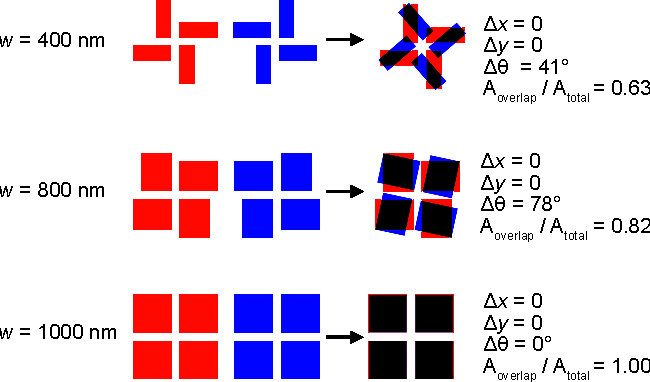
\includegraphics[scale=0.8]{./figures/results/EnantiomorphingChiralCrosses/geoDiff.pdf}
    \caption{\label{fig:appendix:ChiralGeoDiff}
    Examples of the overlap used to define our chiral geometric difference. Red and blue show the right- and left- handed crosses respectively.   $A_{Total}$ is the sum of the red and blue areas. $A_{Overlap}$ is the maximum overlapping area, shown in black. $\Delta x$, $\Delta y$ and $\Delta \theta$ give the parameters for translation ($x$, $y$) and rotation respectively, obtained by maximizing $A_{Overlap}$. In the achiral case ($w=\SI{1000}{\nano\m}$), complete overlap is possible because the structure is achiral. }	
\end{figure}

\section{Scattering Spectra}\label{sec:appendix:CrossesScatteringSpectra}

For additional characterisation of the chiral cross samples (section~\ref{sec:results:EnantiomorphingChiralCrosses}), linear scattering spectra were both simulated and experimentally obtained. In simulations, no significant circular dichroism was observed. In the experimental data, no circular dichroism could be observed above experimental noise.

\begin{figure}[htb!]	
    \centering	
    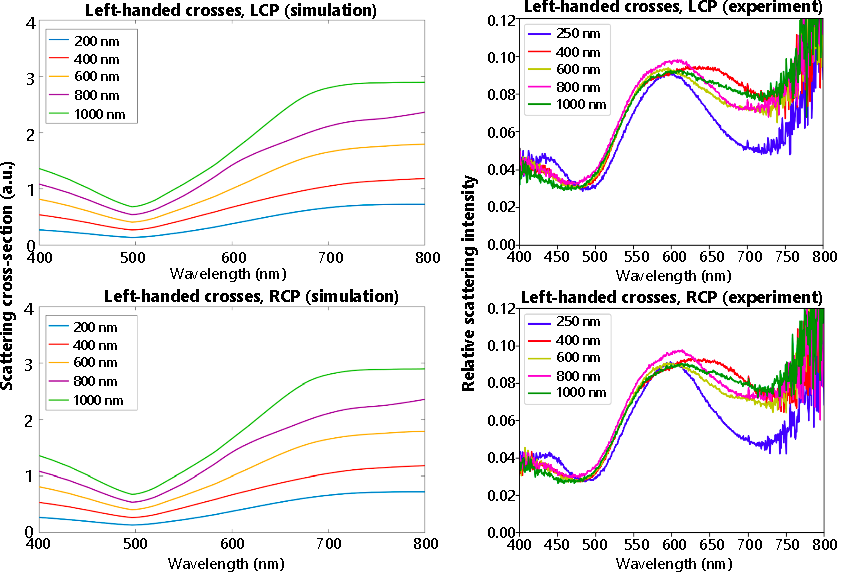
\includegraphics[scale=1.0]{./figures/results/EnantiomorphingChiralCrosses/scattering_data.pdf}
    \caption{\label{fig:appendix:CrossesScatteringSpectra}
    (Left) Numerically-obtained linear scattering cross sections for left-handed chiral cross structures under LCP (top) and RCP (bottom) illumination, with varying arm width (legend). (Right) Experimentally obtained linear scattering spectra for the same structures. }
\end{figure}